\documentclass[11pt,a4paper]{article}

\usepackage[T1]{fontenc}
\usepackage[utf8]{inputenc}
\usepackage{lmodern}
\usepackage{amsmath,amssymb,amsthm}
\usepackage{mathtools}
\usepackage{booktabs}
\usepackage{graphicx}
\usepackage[margin=1.1in]{geometry}
\usepackage{microtype}
\usepackage[htt]{hyphenat}
\setlength{\emergencystretch}{3em}
\usepackage{xcolor}
\definecolor{linkblue}{RGB}{20,60,120}
\usepackage[colorlinks=true,linkcolor=linkblue,citecolor=linkblue,
            urlcolor=linkblue]{hyperref}

\theoremstyle{plain}
\newtheorem{theorem}{Theorem}[section]
\newtheorem{proposition}[theorem]{Proposition}
\newtheorem{lemma}[theorem]{Lemma}
\newtheorem{corollary}[theorem]{Corollary}
\theoremstyle{definition}
\newtheorem{definition}[theorem]{Definition}
\newtheorem{example}[theorem]{Example}
\newtheorem{problem}[theorem]{Problem}
\newtheorem{conjecture}[theorem]{Conjecture}
\theoremstyle{remark}
\newtheorem{remark}[theorem]{Remark}

\newtheorem{theoremA}{Theorem A}
\renewcommand{\thetheoremA}{}
\newtheorem{theoremB}{Theorem B}
\renewcommand{\thetheoremB}{}
\newtheorem{theoremC}{Theorem C}
\renewcommand{\thetheoremC}{}
\newtheorem{theoremD}{Theorem D}
\renewcommand{\thetheoremD}{}
\newtheorem{theoremE}{Theorem E}
\renewcommand{\thetheoremE}{}

\DeclareMathOperator{\lm}{lm}
\DeclareMathOperator{\gs}{gs}
\newcommand{\Fk}{\mathbb{F}_k}
\newcommand{\ovr}{\mathrm{over}}
\newcommand{\undr}{\mathrm{under}}
\newcommand{\Lean}[1]{\texttt{#1}}

\title{The gap series of an integer sequence:\\
an arithmetic invariant governing subset-sum landscapes}
\author{Kentaro Amauchi\thanks{Independent researcher.
\href{mailto:amkn.sub03@gmail.com}{amkn.sub03@gmail.com},
\url{https://mathlab0911.github.io/}}}
\date{\today}

\begin{document}
\maketitle

\begin{abstract}
For a finite sequence $A=(a_1,\dots,a_k)$ of positive integers we introduce the
\emph{gap series} $\Gamma(A)=\sum_{j=1}^{k}a_j2^{-j}\in\mathbb{Q}$, an
order-sensitive invariant equal to the generating function of $A$ evaluated at
$x=1/2$. We show that $\Gamma$ governs the combinatorics of subset sums of $A$.

Fix a target $n$, give the subsets $S$ of $A$ the energy $E(S)=|\sigma(S)-n|$,
where $\sigma$ is the sum, and take single-element flips as moves. Let
$\lm_A(n)$ be the number of strict local minima and $\deg_A(n)$ the number of
ground states. We prove a classification theorem for local minima; a window
identity $W_D(A)=\Gamma(A)+(2D+1)2^{-k}$; and an exact stratification of
$\lm_A(n)$ in which each stratum is a representation count $r_{B_d}$ of a
truncated subsequence. If those representation counts are \emph{flat} to within
a factor $1+\varepsilon$ on an explicit window, then
\[
\frac{W_D(A)}{1+\varepsilon}\;\le\;\frac{\lm_A(n)}{\deg_A(n)}\;\le\;(1+\varepsilon)\,W_D(A).
\]
This replaces the annealed (independence) approximation standard in the
statistical-mechanics literature by a finite, checkable hypothesis.

We complement it with a lower bound. Writing $F_B(z)=\prod_{a\in B}(1+z^{a})$
for the generating polynomial of the representation counts, we show that
$|F_B(i)|=2^{|B|/2}$ exactly for \emph{every} odd sequence $B$ --- the
modulus-$4$ character never degenerates, whereas the modulus-$6$ one vanishes
as soon as $3\in B$. Consequently the representation counts are never
equidistributed modulo $4$: the spread of the residue-class totals is
determined exactly by the parity of $|B|$, and the relative spread is always at
least $2\sqrt2\cdot2^{-|B|/2}$. We also determine which congruence is
responsible: the geometric mean $M(q)$ of $|\cos(\pi r/q)|$ over $r$ coprime to
$q$ equals $\tfrac12|\Phi_q(-1)|^{1/\varphi(q)}$, and $\sup_{q\ge3}M(q)=\sqrt3/2$
is attained at $q=6$ alone. The primes, confined modulo $6$ to the two residues
realising this maximum, sit at rate $\sqrt3/2\approx0.866$ --- above the
universal floor $1/\sqrt2\approx0.707$, so they are among the \emph{least} flat
odd sequences rather than the flattest.

We compute $\varepsilon$ exactly for $k\le32$: for the odd primes it decays
geometrically at rate $\approx\sqrt3/2$, matching the modulus-$6$ prediction to
within $1\%$, while for random odd sequences it decays strictly faster. Over
$100$ random sequences per $k\in\{8,12,16,18,20\}$ we find
$(\lm/\deg)/\Gamma\to1$ with standard deviation $0.0067$ at $k=20$ and
$R^2=0.999$. A partial-correlation analysis shows that $\Gamma$ subsumes the
coefficient of variation of the weights, the statistic previously proposed for
this role by Alyahya and Rowe.

All theorems below are formally verified in Lean~4 with Mathlib; no proof
contains \Lean{sorry} and no additional axiom is used. The development is
available at \url{https://github.com/mathlab0911/arithmetic-landscape}.
\end{abstract}

\noindent\textbf{2020 MSC.} 11B75 (primary); 05A17, 68Q25, 82B44.

\noindent\textbf{Keywords.} gap series, subset sums, number partitioning,
local minima, energy landscape, primes, formal verification.

\tableofcontents

\section{Introduction}

\subsection{The gap series}

Let $A=(a_1,\dots,a_k)$ be a finite sequence of positive integers. Its
\emph{gap series} is
\[
  \Gamma(A)\;=\;\sum_{j=1}^{k}\frac{a_j}{2^{j}}.
\]

Two elementary remarks fix the character of this quantity.

First, $\Gamma$ is \emph{order-sensitive}. It is not a function of the multiset
$\{a_1,\dots,a_k\}$: reordering the sequence changes its value. This
distinguishes $\Gamma$ from the statistics ordinarily attached to a set of
weights --- mean, variance, coefficient of variation --- all of which are
order-blind.

Second, writing $a_0=0$ and summing by parts,
\[
  \Gamma(A)\;=\;\sum_{j=0}^{k-1}\frac{a_{j+1}-a_j}{2^{j}}\;-\;\frac{a_k}{2^{k}},
\]
so that for an increasing sequence $\Gamma$ is a dyadically weighted sum of the
\emph{gaps} of $A$, dominated by the earliest ones. For the odd primes
$3,5,7,11,\dots$ the small initial gaps --- in particular the twin pairs
$(3,5)$, $(5,7)$, $(11,13)$, $(17,19)$ --- force $\Gamma$ to be small:
$\Gamma(3,5,\dots,73)=5609051/1048576\approx5.3492$, against $\approx8.09$ on
average for a random odd sequence of the same length drawn from the same range.

The purpose of this paper is to show that this innocuous-looking quantity
controls a genuinely combinatorial object: the local structure of the
subset-sum problem for $A$.

\begin{remark}[Terminology]
The name is meant to record the second formula above: $\Gamma$ is a dyadically
weighted series in the gaps of $A$. It should not be confused with the
\emph{gap-sum sequence} of an integer sequence in the sense of Barry~\cite{Ba21},
which is formed from the integers \emph{absent} between consecutive terms; that
construction and ours share no content beyond the word ``gap''.
Readers who prefer an unambiguous name may read $\Gamma$ as the
\emph{dyadic gap series}, or simply as the generating function of $A$ evaluated
at $x=1/2$.
\end{remark}

\subsection{Subset-sum landscapes}

Fix a target $n\in\mathbb{N}$. For $S\subseteq\{1,\dots,k\}$ put
$\sigma(S)=\sum_{i\in S}a_i$ and $E(S)=|\sigma(S)-n|$. Two configurations are
adjacent if they differ in a single index. This is the standard $1$-bit-flip
landscape of the number partitioning problem (NPP); the case
$n=\sigma(A)/2$ is the balanced partition problem. We study
\[
  \deg_A(n)=\#\{S: E(S)=0\},
  \qquad
  \lm_A(n)=\#\{S: E(S)<E(S')\ \text{for all neighbours }S'\}.
\]
Here $\lm$ counts the \emph{valleys} of the landscape and is the standard
measure of its ruggedness.

Our main results are the following; full statements appear in the sections
indicated.

\begin{theoremA}[Classification; \S\ref{sec:classification}]
Suppose all $a_i>0$ and let $d=E(S)$. If $\sigma(S)\ge n$, then $S$ is a strict
local minimum if and only if $a_i>2d$ for every $i\in S$. If $\sigma(S)\le n$,
then $S$ is a strict local minimum if and only if $a_i>2d$ for every $i\notin S$.
\end{theoremA}

Thus membership in the set of local minima is decided by a condition involving
only the elements of size at most $2d$; everything larger is irrelevant. This is
the engine of the whole paper.

\begin{theoremB}[Window identity; \S\ref{sec:window}]
Let $A$ be non-decreasing with all $a_i$ odd and $a_i\le2D+1$. Put
$N_A(d)=\#\{i:a_i\le2d\}$ and $W_D(A)=1+2\sum_{d=1}^{D}2^{-N_A(d)}$. Then
\[
  W_D(A)\;=\;\Gamma(A)+\frac{2D+1}{2^{k}}.
\]
\end{theoremB}

The quantity $W_D$ is the total measure of the ``windows'' in which a
configuration at error $d$ can be a local minimum, computed as if the elements
were placed independently. Theorem~B says that this measure is exactly the gap
series, up to a tail term negligible for the sequences of interest
($73/2^{20}\approx7\times10^{-5}$ for the first twenty odd primes).

\begin{theoremC}[Exact stratification; \S\ref{sec:stratification}]
Without any approximation,
\[
  \lm_A(n)\;=\;\deg_A(n)+\sum_{d\ge1}\bigl(\ovr_A(n,d)+\undr_A(n,d)\bigr),
\]
where the strata vanish once $2d$ exceeds $\max_i a_i$, and each stratum equals
a representation count of a truncated subsequence,
\[
  \ovr_A(n,d)=r_{B_d}(n+d),
  \qquad
  \undr_A(n,d)=r_{B_d}\bigl(n-d-\sigma(I_d)\bigr),
\]
with $I_d=\{i:a_i\le2d\}$ and $B_d=A|_{I_d^{c}}$. Moreover
$\deg_A(n)=\sum_{J\subseteq I_d}r_{B_d}(n-\sigma(J))$.
\end{theoremC}

\begin{theoremD}[Sandwich; \S\ref{sec:sandwich}]
Suppose that for every $d\le D$ the representation counts $r_{B_d}$ vary by at
most a factor $1+\varepsilon$ across the window
$\{n-\sigma(J):J\subseteq I_d\}\cup\{n+d,\;n-d-\sigma(I_d)\}$. Then
\[
  \frac{W_D(A)}{1+\varepsilon}\;\le\;\frac{\lm_A(n)}{\deg_A(n)}\;\le\;(1+\varepsilon)\,W_D(A).
\]
\end{theoremD}

Combining Theorems~B and~D, $\lm/\deg$ is pinned to $\Gamma(A)$ with a
multiplicative error controlled by a single, explicitly computable number
$\varepsilon$.

The flatness $\varepsilon$ cannot be made to vanish arbitrarily fast. Write
$F_B(z)=\prod_{a\in B}(1+z^{a})$, so the representation counts $r_B$ are the
coefficients of $F_B$, and let $R_c=\sum_{m\equiv c\,(4)}r_B(m)$.

\begin{theoremE}[Universal obstruction; \S\ref{sec:floor}]
For every finite sequence $B$ of odd positive integers, $|F_B(i)|=2^{|B|/2}$
exactly, whatever the residues of the elements. Consequently the counts $R_c$
are never all equal; their spread is determined by the parity of $|B|$,
\[
  \max_c R_c-\min_c R_c=2^{|B|/2}\ \ (|B|\text{ even}),
  \qquad 2^{(|B|-1)/2}\ \ (|B|\text{ odd}),
\]
so the relative spread is always at least $2\sqrt2\cdot2^{-|B|/2}$.
\end{theoremE}

This is a lower bound, in contrast with Theorems~B--D, and it is elementary:
$1+i^{a}=1\pm i$ has modulus $\sqrt2$ for \emph{every} odd $a$, so the
modulus-$4$ character never degenerates. The modulus-$6$ character does: if
$3\in B$ then $F_B(\zeta_6)=0$.

The obstruction of Theorem~E is a statement about the distribution of $r_B$
across residue classes modulo $4$, not about the pointwise flatness
$\varepsilon_d$ of Theorem~D; we do not derive a lower bound for the latter,
and \S\ref{sec:floor} explains why the transfer needs an input we do not have.
Numerically, however, the two sit at the same scale for random odd sequences,
whereas for the primes $\varepsilon_2$ exceeds the modulus-$4$ scale by two
orders of magnitude at $k=32$: their obstruction decays at rate
$\sqrt3/2\approx0.866$, against $1/\sqrt2\approx0.707$. In that sense the
primes are not the flattest odd sequences but among the least flat.

We emphasise what Theorem~D does \emph{not} assume. The statistical-mechanics
treatment of the NPP proceeds through the annealed approximation, in which
configurations are treated as independent. Theorems~C and~D dispense with this:
the decomposition is an identity, and the only input is the flatness of an
explicit arithmetic function on an explicit finite window. Flatness is not an
idealisation --- it is a quantity one can compute for any given $A$, and we do
so in \S\ref{sec:flatness-measured}.

\subsection{Relation to previous work}

The NPP has been studied intensively from the statistical-mechanics side.
Ferreira and Fontanari~\cite{FF98} analysed the problem for i.i.d.\ weights
uniform on $[0,1]$, identifying it with the ground-state problem for an
infinite-range antiferromagnetic Ising model, and computed within the annealed
approximation the fraction of metastable states --- configurations stable under
all single spin flips --- showing that it vanishes like $N^{-3/2}$.
Mertens~\cite{Me01} surveys the physicist's approach; Stadler, Hordijk and
Fontanari~\cite{SHF03} study landscape statistics across the phase transition;
and Borgs, Chayes and Pittel~\cite{BCP01} give a rigorous treatment of the
transition and its finite-size scaling.

We stress that \emph{the order of magnitude $2^{k}k^{-3/2}$ for the number of
local minima of a random instance is not new here}. It is exactly the content of
the annealed computation of~\cite{FF98}. Our contribution lies elsewhere, in two
directions.

\emph{Deterministic sequences.} The literature treats the weights as random and
asks for typical behaviour. We fix a deterministic sequence --- for instance the
primes --- and ask which of its \emph{arithmetic} features control the
landscape. The answer, Theorems~B--D, is the gap series, an invariant with no
probabilistic content.

\emph{Exactness.} The annealed approximation is replaced by an identity plus a
checkable hypothesis. To our knowledge Theorem~C, and the reduction of
$\lm/\deg$ to the flatness of truncated representation counts, are new.

The closest precursor is Alyahya and Rowe~\cite{AR14}, who observed empirically
that the number of local optima in the $1$-bit-flip NPP landscape is strongly
\emph{negatively} correlated with the coefficient of variation $CV$ of the
weights, and proposed an estimator based on $CV$. Their observation is correct
and we reproduce it (\S\ref{sec:cv}). But $CV$ is order-blind while $\Gamma$ is
not, and Theorem~B shows it is $\Gamma$, not $CV$, that equals the window
measure $W_D$. Partial-correlation analysis on $100$ instances per size confirms
the theoretical expectation: conditioning on $CV$ leaves the $\Gamma$-correlation
essentially intact, while conditioning on $\Gamma$ removes almost all of the
$CV$-correlation. In this precise sense $\Gamma$ subsumes $CV$.

\subsection{Formal verification}

Every theorem stated in \S\S\ref{sec:definitions}--\ref{sec:sandwich} has been
formalised in Lean~4 against Mathlib. Each formal statement is accompanied in
the text by the name of the corresponding Lean declaration, and
Appendix~\ref{app:lean} lists the files, the declarations and the reproduction
procedure. We have verified with \Lean{\#print axioms} that no declaration
depends on \Lean{sorryAx} or on any axiom beyond Lean's standard
\Lean{propext}, \Lean{Classical.choice} and \Lean{Quot.sound}.

Two remarks on what this did and did not buy us. It did not merely confirm
proofs already written on paper: formalisation of Theorem~D revealed that the
exponent could be improved from $(1+\varepsilon)^{\pm2}$ to
$(1+\varepsilon)^{\pm1}$, since numerator and denominator may be controlled by
the same flatness estimate. On the other hand, formalisation forced us to state
hypotheses that are easy to leave implicit --- most notably the non-decreasing
hypothesis in Theorem~B, whose necessity we exhibit by a two-element
counterexample in \S\ref{sec:order-matters}.

\section{Definitions, and the bridge to computation}\label{sec:definitions}

\subsection{The landscape}

Throughout, $A$ denotes a finite sequence of positive integers, presented either
as a list $(a_1,\dots,a_k)$ or as a function $A:\Fk\to\mathbb{N}$ on the index
type $\Fk=\{0,\dots,k-1\}$; \S\ref{sec:bridge} shows the two presentations
agree. We write $\sigma(S)=\sum_{i\in S}a_i$ for $S\subseteq\Fk$, and
$T=\sigma(A)$. For a target $n$,
\[
  E_n(S)=|\sigma(S)-n|,
  \qquad
  \operatorname{flip}(S,i)=
  \begin{cases}S\setminus\{i\}&i\in S,\\ S\cup\{i\}&i\notin S,\end{cases}
\]
and $S$ is a \emph{strict local minimum} if $E_n(S)<E_n(\operatorname{flip}(S,i))$
for all $i$. We set
\[
  \gs_A(n)=\min_S E_n(S),\quad
  \deg_A(n)=\#\{S:\sigma(S)=n\},\quad
  \lm_A(n)=\#\{S:S\text{ strict local min}\}.
\]
(Lean: \Lean{ndist}, \Lean{subsetSums}, \Lean{gs}, \Lean{energy}, \Lean{flip},
\Lean{IsStrictLocalMin}, \Lean{lm}, \Lean{degCount}.)

\subsection{The bridge}\label{sec:bridge}

Implementations enumerate subsets by bitmasks over a list; proofs are more
convenient over $\operatorname{Finset}(\Fk)$. That these describe the same object
is not automatic, and we record it.

\begin{proposition}\label{prop:bridge}
For $A:\Fk\to\mathbb{N}$ and $s\in\mathbb{N}$,
$s\in\operatorname{subsetSums}(\operatorname{ofFn}A)$ if and only if there exists
$S\subseteq\Fk$ with $\sigma(S)=s$.
\textup{(Lean: \Lean{mem\_subsetSums\_ofFn\_iff}.)}
\end{proposition}

\begin{proposition}\label{prop:gs-min}
$\gs_A(n)$ equals $\min_S E_n(S)$, and the minimum is attained.
\textup{(Lean: \Lean{gs\_ofFn\_eq\_energy\_min}.)}
\end{proposition}

\begin{proposition}[Representability]\label{prop:representability}
$\gs_A(n)=0$ if and only if $n$ is a sum of a sub-sequence of $A$.
\textup{(Lean: \Lean{gs\_eq\_zero\_iff}.)}
\end{proposition}

Proposition~\ref{prop:representability} is the translation used throughout: the
statement ``the landscape has ground energy zero'' is the statement ``$n$ is
representable'', and $\deg_A(n)$ is the number of representations, denoted
$r_A(n)$ below.

\section{The classification theorem}\label{sec:classification}

\begin{theorem}[Classification]\label{thm:classification}
Let $a_i>0$ for all $i$, let $S\subseteq\Fk$ and $d=E_n(S)$.
\begin{enumerate}
\item If $\sigma(S)\ge n$: $S$ is a strict local minimum
      $\iff$ $a_i>2d$ for all $i\in S$.
\item If $\sigma(S)\le n$: $S$ is a strict local minimum
      $\iff$ $a_i>2d$ for all $i\notin S$.
\end{enumerate}
\textup{(Lean: \Lean{isStrictLocalMin\_iff\_of\_ge},
\Lean{isStrictLocalMin\_iff\_of\_le}, combined form
\Lean{isStrictLocalMin\_iff\_classCond}.)}
\end{theorem}

\begin{proof}
Suppose $\sigma(S)=n+d$ with $d\ge0$. Removing $i\in S$ changes the sum to
$n+d-a_i$, whose error is $|d-a_i|$; this is $\ge d$ precisely when $a_i\ge2d$,
and $>d$ precisely when $a_i>2d$. Adding $i\notin S$ only increases the error,
since $a_i>0$. The deficient case is symmetric.
\end{proof}

We claim no originality for Theorem~\ref{thm:classification}: the computation is
immediate, and some form of it is presumably known to anyone who has looked at
the $1$-bit-flip landscape of the NPP, though we have not located an explicit
statement in the literature. We record it here because everything below is built
on it, and because the formal development requires a precise version. What we do
claim is the use made of it in \S\S\ref{sec:window}--\ref{sec:sandwich}.

\begin{corollary}\label{cor:ground-is-min}
A ground state ($d=0$) is always a strict local minimum.
\textup{(Lean: \Lean{isStrictLocalMin\_of\_exact}.)}
\end{corollary}

\begin{corollary}\label{cor:lm-arithmetic}
$\lm_A(n)$ equals the number of $S$ satisfying the arithmetic condition of
Theorem~\ref{thm:classification}; in particular $\lm$ is a counting function of
the sequence and target alone.
\textup{(Lean: \Lean{lm\_eq\_lmClassCount}.)}
\end{corollary}

The force of Theorem~\ref{thm:classification} is a \emph{locality} statement:
whether $S$ is a valley depends only on the elements of $A$ that are at most
$2d$, where $d$ is the error at $S$. Since a landscape has few configurations at
large error, and the constraint at error $d$ involves
$N_A(d)=\#\{i:a_i\le2d\}$ elements, the count of valleys is governed by how
quickly $N_A(d)$ grows --- that is, by the early gaps of $A$. Sections
\ref{sec:window}--\ref{sec:sandwich} make this precise.

\section{Symmetry and parity}\label{sec:symmetry}

Throughout this section $T=\sigma(A)$.

\begin{theorem}[Reflection]\label{thm:reflection}
For $n\le T$: $\gs_A(T-n)=\gs_A(n)$ and $\lm_A(T-n)=\lm_A(n)$.
\textup{(Lean: \Lean{gs\_compl}, \Lean{lm\_compl}.)}
\end{theorem}

\begin{proof}
The map $S\mapsto S^{c}$ is an involution of the configuration space satisfying
$\sigma(S^{c})=T-\sigma(S)$, hence $E_{T-n}(S^{c})=E_n(S)$; and it commutes with
single-element flips, $\operatorname{flip}(S,i)^{c}=\operatorname{flip}(S^{c},i)$.
So it carries strict local minima for target $n$ bijectively onto those for
target $T-n$.
\end{proof}

\begin{theorem}[No flat edges]\label{thm:no-flat}
If every $a_i$ is odd, then $E_n(S)\ne E_n(\operatorname{flip}(S,i))$ for all $S$
and $i$. \textup{(Lean: \Lean{no\_flat\_edge}.)}
\end{theorem}

\begin{proof}
$|x-n|\equiv x+n\pmod2$, and flipping $i$ changes $\sigma(S)$ by the odd number
$a_i$, hence changes the parity of the error.
\end{proof}

\begin{corollary}\label{cor:strict-eq-weak}
For odd $A$, strict local minima and weak local minima coincide.
\textup{(Lean: \Lean{isStrictLocalMin\_iff\_le\_of\_odd}.)}
\end{corollary}

Corollary~\ref{cor:strict-eq-weak} is the reason we restrict to odd sequences:
for such $A$ --- and the odd primes are the motivating example --- the quantity
$\lm_A(n)$ does not depend on which of the two standard definitions of ``local
minimum'' one adopts. For sequences containing even elements the landscape has
plateaus and the two counts genuinely differ.

\section{The window identity}\label{sec:window}

\subsection{Windows}

By Theorem~\ref{thm:classification}, a configuration at error $d$ is a local
minimum precisely when the $N_A(d)$ elements of size $\le2d$ all lie on a
prescribed side. If the elements were placed independently and uniformly, the
proportion of configurations satisfying this would be $2^{-N_A(d)}$. Summing
over $d$, with the excess and deficient sides contributing separately and the
ground level ($d=0$) once, gives the \emph{window series}
\[
  W_D(A)\;=\;1+2\sum_{d=1}^{D}2^{-N_A(d)},
  \qquad N_A(d)=\#\{i:a_i\le2d\}.
\]
(Lean: \Lean{winCount}, \Lean{windowSum}, \Lean{windowSeries}; the $\Fk$ version
is \Lean{winCountFin}, \Lean{winSeriesFin}.)

$W_D$ is the annealed prediction for $\lm_A(n)/\deg_A(n)$. Sections
\ref{sec:stratification}--\ref{sec:sandwich} show in what exact sense it is
correct; the present section evaluates it.

\subsection{The identity}

\begin{theorem}\label{thm:window}
Let $A$ be a non-decreasing sequence of odd positive integers with $a_i\le2D+1$
for all $i$. Then
\[
  W_D(A)\;=\;\Gamma(A)+\frac{2D+1}{2^{k}}.
\]
\textup{(Lean: \Lean{windowSeries\_eq\_gapSeries}.)}
\end{theorem}

\begin{proof}
Induction on the length of $A$, the inductive step resting on the pointwise
identity
\[
  2^{-N_{a:t}(d)}\;=\;\tfrac12\Bigl(2^{-N_{t}(d)}+\mathbf 1[\,2d<a\,]\Bigr),
\]
valid when $a\le b$ for all $b\in t$ (Lean: \Lean{window\_term\_cons}). Indeed
if $a\le2d$ then $N_{a:t}(d)=N_t(d)+1$ and the indicator vanishes; if $2d<a$
then no element of $a:t$ is $\le2d$, so both sides equal $1$. Summing over
$d\in[1,D]$ and using $\#\{d\le D:2d<a\}=\lfloor a/2\rfloor$ (here $a\le2D+1$ is
used) gives
\[
  \sum_{d=1}^{D}2^{-N_{a:t}(d)}
  =\tfrac12\Bigl(\sum_{d=1}^{D}2^{-N_t(d)}+\lfloor a/2\rfloor\Bigr),
\]
whence $W_D(a:t)=1+\lfloor a/2\rfloor+\tfrac12(W_D(t)-1)$. Substituting the
inductive hypothesis $W_D(t)=\Gamma(t)+(2D+1)2^{-|t|}$ and using
$\lfloor a/2\rfloor=(a-1)/2$ for odd $a$, together with
$\Gamma(a:t)=\tfrac a2+\tfrac{\Gamma(t)}2$, gives the claim. The base case
$A=\varnothing$ reads $1+2D=0+(2D+1)$.
\end{proof}

Note that $D$ may be taken arbitrarily large: increasing $D$ adds terms $2^{-k}$
on the left, absorbed exactly by the tail term on the right. The natural choice
for an increasing sequence is $D=(a_k-1)/2$, the smallest value for which all
elements are $\le2D+1$; then $W(A)=\Gamma(A)+a_k2^{-k}$, and for the first
twenty odd primes the correction is $73/2^{20}\approx6.96\times10^{-5}$.

\subsection{Order matters}\label{sec:order-matters}

$W_D$ depends only on the multiset underlying $A$, whereas $\Gamma$ depends on
the order. Theorem~\ref{thm:window} can therefore hold only for one ordering,
and it is worth exhibiting the failure explicitly.

\begin{example}\label{ex:order}
Take $A=(5,3)$ and $D=2$. Then $N_A(1)=0$ and $N_A(2)=1$, so
$W_2(A)=1+2(1+\tfrac12)=4$, while $\Gamma(A)=\tfrac52+\tfrac34=\tfrac{13}4$ and
$\Gamma(A)+\tfrac{5}{4}=\tfrac92\ne4$. Reordering to $(3,5)$ restores the
identity: $\Gamma=\tfrac32+\tfrac54=\tfrac{11}4$ and
$\tfrac{11}4+\tfrac54=4$. Both computations are \Lean{\#eval}-checked in the
Lean development.
\end{example}

We return to this in \S\ref{sec:cv}: it is precisely the order-sensitivity of
$\Gamma$ that separates it from order-blind statistics such as the coefficient
of variation, and Example~\ref{ex:order} is the shortest demonstration that no
order-blind statistic can play the role of $\Gamma$ in
Theorem~\ref{thm:window}.

\section{Exact stratification}\label{sec:stratification}

\subsection{Strata}

Fix $A$ with $a_i>0$ and a target $n$. Following
Theorem~\ref{thm:classification}, define for $d\ge0$
\begin{align*}
  \ovr_A(n,d)&=\#\{S:\sigma(S)=n+d,\ \forall i\in S,\ a_i>2d\},\\
  \undr_A(n,d)&=\#\{S:\sigma(S)+d=n,\ \forall i\notin S,\ a_i>2d\}.
\end{align*}
(Lean: \Lean{overCount}, \Lean{underCount}.)

\begin{lemma}\label{lem:fibers}
The set of strict local minima with $\sigma(S)=s$ has cardinality
$\ovr_A(n,s-n)$ if $s\ge n$, and $\undr_A(n,n-s)$ if $s<n$.
\textup{(Lean: \Lean{fiber\_over}, \Lean{fiber\_under}.)}
\end{lemma}

\begin{lemma}\label{lem:vanishing}
$\ovr_A(n,0)=\undr_A(n,0)=\deg_A(n)$. If $a_i\le2d$ for all $i$ and $d\ge1$,
then $\ovr_A(n,d)=\undr_A(n,d)=0$.
\textup{(Lean: \Lean{overCount\_zero\_eq\_degCount},
\Lean{underCount\_zero\_eq\_degCount}, \Lean{overCount\_eq\_zero},
\Lean{underCount\_eq\_zero}.)}
\end{lemma}

\begin{theorem}[Exact stratification]\label{thm:stratification}
For $n\le T$ and any $D$ with $a_i\le2D+1$ for all $i$,
\[
  \lm_A(n)\;=\;\deg_A(n)\;+\;\sum_{d=1}^{D}\bigl(\ovr_A(n,d)+\undr_A(n,d)\bigr).
\]
\textup{(Lean: \Lean{lm\_eq\_sum\_strata} in the sum-indexed form;
\Lean{lm\_eq\_lmPartial} and \Lean{lm\_eq\_lmPartial\_of\_le} in the
$d$-indexed form used here.)}
\end{theorem}

\begin{proof}
Fibring the set of strict local minima over the value $\sigma(S)\in[0,T]$ and
applying Lemma~\ref{lem:fibers} gives the sum-indexed identity. Re-indexing the
excess part by $d=s-n$ and the deficient part by $d=n-s$ (the latter via
reflection of a range sum), then extracting the $d=0$ term and truncating both
sums at $D$ using Lemma~\ref{lem:vanishing}, gives the stated form.
\end{proof}

We stress that Theorem~\ref{thm:stratification} is an identity between integers.
No independence assumption enters.

\subsection{Strata are representation counts}

Write $I_d=\{i:a_i\le2d\}$, $N(d)=|I_d|$, $\sigma_d=\sigma(I_d)$, and let $B_d$
be the subsequence of $A$ indexed by $I_d^{c}$. As in \S\ref{sec:bridge},
$r_{B}(m)$ denotes the number of subsets of $B$ summing to $m$.

\begin{theorem}[Fibres]\label{thm:fiber-rep}
Let $J\subseteq I$. Then
\[
  \#\{S:\sigma(S)=n,\ S\cap I=J\}\;=\;r_{A|_{I^{c}}}\bigl(n-\sigma(J)\bigr).
\]
\textup{(Lean: \Lean{fiber\_card\_eq\_repCount}; the bijection is
$S\mapsto S\setminus I$, with inverse $U\mapsto U\cup J$.)}
\end{theorem}

\begin{corollary}\label{cor:deg-rep}
$\deg_A(n)=\sum_{J\subseteq I}r_{A|_{I^{c}}}(n-\sigma(J))$ for any $I$.
\textup{(Lean: \Lean{degCount\_eq\_sum\_repCount}, combining
Theorem~\ref{thm:fiber-rep} with \Lean{degCount\_fiberwise}.)}
\end{corollary}

\begin{corollary}\label{cor:strata-rep}
$\ovr_A(n,d)=r_{B_d}(n+d)$ and, for $d\le n$,
$\undr_A(n,d)=r_{B_d}(n-d-\sigma_d)$.
\textup{(Lean: \Lean{overCount\_eq\_repCount},
\Lean{underCount\_eq\_repCount}; these are Theorem~\ref{thm:fiber-rep} with
$J=\varnothing$ and $J=I_d$ respectively.)}
\end{corollary}

\subsection{What has been achieved}

Combining the above,
\[
  \frac{\lm_A(n)}{\deg_A(n)}
  \;=\;1+\sum_{d=1}^{D}
  \frac{r_{B_d}(n+d)+r_{B_d}(n-d-\sigma_d)}
       {\sum_{J\subseteq I_d}r_{B_d}(n-\sigma(J))}.
\]
Every quantity on the right is a representation count of a truncated
subsequence of $A$. The ratio of valleys to ground states has been expressed
\emph{exactly} in terms of the arithmetic function $r$, with no probabilistic
input whatever.

The denominator is a sum of $2^{N(d)}$ values of $r_{B_d}$ at the points
$n-\sigma(J)$, $J\subseteq I_d$; the numerator consists of two further values of
the same function. If $r_{B_d}$ were constant on the window spanned by these
$2^{N(d)}+2$ points, the $d$-th summand would equal exactly $2\cdot2^{-N(d)}$
and the total would be exactly $W_D(A)=\Gamma(A)+(2D+1)2^{-k}$ by
Theorem~\ref{thm:window}.

The annealed approximation of the physics literature is thus revealed to be
exactly the assertion that $r_{B_d}$ is constant on this window. It is not; but
it is nearly so, and ``nearly'' is quantifiable. That is the content of
\S\ref{sec:sandwich}.

\section{Flatness and the sandwich}\label{sec:sandwich}

\subsection{The abstract lemma}

\begin{lemma}\label{lem:flat-ratio}
Let $s$ be a finite non-empty index set, $g:s\to\mathbb{Q}_{>0}$,
$v\in\mathbb{Q}_{>0}$ and $\varepsilon\ge0$. If $g(i)\le(1+\varepsilon)v$ and
$v\le(1+\varepsilon)g(i)$ for all $i\in s$, then
\[
  \frac{1}{(1+\varepsilon)\,|s|}\;\le\;\frac{v}{\sum_{i\in s}g(i)}\;\le\;\frac{1+\varepsilon}{|s|}.
\]
\textup{(Lean: \Lean{ratio\_bounds\_of\_flat}.)}
\end{lemma}

\begin{proof}
$\sum g\ge|s|\,v/(1+\varepsilon)$ gives the upper bound;
$\sum g\le|s|(1+\varepsilon)v$ gives the lower.
\end{proof}

Elementary as it is, Lemma~\ref{lem:flat-ratio} is the whole mechanism: it
converts flatness of a family into a bound on the share of any one member.

\subsection{The sandwich}

\begin{definition}\label{def:flat}
Say $A$ is \emph{$\varepsilon$-flat at $(n,d)$} if
$r_{B_d}(m')\le(1+\varepsilon)r_{B_d}(m)$ for all $m,m'\in\mathrm{Win}_d$, where
\[
  \mathrm{Win}_d=\{n-\sigma(J):J\subseteq I_d\}\cup\{n+d,\ n-d-\sigma_d\}.
\]
\end{definition}

\begin{theorem}[Sandwich]\label{thm:sandwich}
Let $a_i>0$ be odd, $n\le T$, and let $D$ satisfy $a_i\le2D+1$ for all $i$.
Suppose $\deg_A(n)>0$ and $A$ is $\varepsilon$-flat at $(n,d)$ for every
$1\le d\le D$. Then
\[
  \frac{W_D(A)}{1+\varepsilon}\;\le\;\frac{\lm_A(n)}{\deg_A(n)}\;\le\;(1+\varepsilon)\,W_D(A),
\]
and by Theorem~\ref{thm:window} the outer terms equal
$\bigl(\Gamma(A)+(2D+1)2^{-k}\bigr)(1+\varepsilon)^{\mp1}$.
\textup{(Lean: \Lean{stratum\_ratio\_bounds}, \Lean{sandwich\_partial},
\Lean{sandwich\_total}.)}
\end{theorem}

\begin{proof}
Fix $d$. By Corollary~\ref{cor:deg-rep} the denominator $\deg_A(n)$ is the sum
of the $2^{N(d)}$ numbers $r_{B_d}(n-\sigma(J))$, all of which lie within a
factor $1+\varepsilon$ of $\ovr_A(n,d)=r_{B_d}(n+d)$ by $\varepsilon$-flatness.
Lemma~\ref{lem:flat-ratio} gives
\[
  \frac{2^{-N(d)}}{1+\varepsilon}\;\le\;\frac{\ovr_A(n,d)}{\deg_A(n)}\;\le\;(1+\varepsilon)\,2^{-N(d)},
\]
and the same for $\undr$. Summing over $1\le d\le D$ and adding the $d=0$ term
$\deg/\deg=1$, then invoking Theorem~\ref{thm:stratification}, gives the result;
the elementary inequalities $1\le1+\varepsilon$ and $(1+\varepsilon)^{-1}\le1$
absorb the ground term.
\end{proof}

\begin{remark}
The exponent is $(1+\varepsilon)^{\pm1}$, not $(1+\varepsilon)^{\pm2}$ as a
first analysis suggests, because the same flatness hypothesis controls numerator
and denominator simultaneously. We record this because it was found only in the
course of formalising the argument.
\end{remark}

\begin{remark}
Theorem~\ref{thm:sandwich} is a finite statement over $\mathbb{Q}$. For any
explicit $A$, $n$, $D$ and $\varepsilon$ all quantities are computable, so the
theorem yields certified error bounds for individual instances rather than an
asymptotic statement. The asymptotic question --- whether $\varepsilon$ may be
taken to $0$ as $k\to\infty$ --- is the subject of
\S\ref{sec:flatness-measured} and \S\ref{sec:open}.
\end{remark}

\subsection{A universal obstruction to flatness}\label{sec:floor}

Before measuring $\varepsilon$ we record a lower bound for it, valid for every
odd sequence and proved by an entirely elementary character computation. Recall
$F_B(z)=\prod_{a\in B}(1+z^{a})$ and set $b=|B|$ and
$R_c=\sum_{m\equiv c\,(4)}r_B(m)$ for $c\in\mathbb{Z}/4$.

\begin{theorem}[Universal modulus-$4$ obstruction]\label{thm:floor}
Let $B$ be any finite sequence of odd positive integers, $b=|B|$. Then
\begin{enumerate}
\item $|F_B(i)|=2^{b/2}$, exactly, independently of the residues of the elements
      of $B$; in particular $F_B(i)\ne0$. More precisely
      $F_B(i)=2^{b/2}e^{i\pi(p-q)/4}$ where $p=\#\{a\in B:a\equiv1\,(4)\}$ and
      $q=\#\{a\in B:a\equiv3\,(4)\}$.
\item The spread of the residue-class totals is given \emph{exactly} by the
      parity of $b$:
      \[
        \max_c R_c-\min_c R_c=
        \begin{cases} 2^{b/2} & b \text{ even},\\[2pt] 2^{(b-1)/2} & b \text{ odd}.\end{cases}
      \]
\item Since $\sum_c R_c=2^{b}$, the relative spread equals $4\cdot2^{-b/2}$ for
      $b$ even and $2\sqrt2\cdot2^{-b/2}$ for $b$ odd; in either case
      \[
        \frac{\max_c R_c-\min_c R_c}{\frac14\sum_c R_c}\;\ge\;2\sqrt2\cdot2^{-b/2}.
      \]
\end{enumerate}
\textup{(Lean: \Lean{normSq\_one\_add\_I\_pow\_odd}, \Lean{max\_abs\_cos\_sin\_sq\_ge},
\Lean{spread\_lower\_bound} give (i) and the inequality in (iii).)}
\end{theorem}

\begin{proof}
(i) For odd $a$ we have $i^{a}=\pm i$, so $1+i^{a}$ is $1+i$ or $1-i$ according
as $a\equiv1$ or $3\pmod4$; both have modulus $\sqrt2$, and
$1\pm i=\sqrt2\,e^{\pm i\pi/4}$. Multiplying over $B$ gives
$F_B(i)=2^{b/2}e^{i\pi(p-q)/4}$.

(ii) By discrete Fourier inversion on $\mathbb{Z}/4$,
\[
  R_c=\tfrac14\sum_{j=0}^{3}i^{-jc}F_B(i^{j})
     =\tfrac14\Bigl(2^{b}+2\,\mathrm{Re}\bigl(i^{-c}F_B(i)\bigr)\Bigr),
\]
because $F_B(1)=2^{b}$ and $F_B(-1)=\prod_{a\in B}(1+(-1)^{a})=0$, every $a$
being odd. Writing $\varphi=\pi(p-q)/4$, the quantity
$\mathrm{Re}(i^{-c}F_B(i))/2^{b/2}$ runs over
$\{\cos\varphi,\sin\varphi,-\cos\varphi,-\sin\varphi\}$ as $c$ runs over
$\mathbb{Z}/4$, so the spread is $2^{b/2}\cdot2\max(|\cos\varphi|,|\sin\varphi|)/2$.
By (i) $\varphi$ is a multiple of $\pi/4$, and $p+q=b$ forces
$p-q\equiv b\pmod2$. If $b$ is even then $\varphi$ is a multiple of $\pi/2$ and
$\max(|\cos\varphi|,|\sin\varphi|)=1$; if $b$ is odd then $\varphi$ is an odd
multiple of $\pi/4$ and the maximum is $1/\sqrt2$. This gives the two cases.

(iii) Divide by $\tfrac14\sum_cR_c=2^{b-2}$.
\end{proof}

The identity in (ii) is worth emphasising: the spread is not merely bounded
below, it is \emph{determined}, and only by the parity of $b$ --- the residues
of the individual elements are irrelevant. We have checked it numerically for
the truncated prime sequences and for random odd sequences up to $k=32$, where
the ratio of the measured relative spread to $2\sqrt2\cdot2^{-b/2}$ is exactly
$1$ when $b$ is odd and exactly $\sqrt2$ when $b$ is even, with no intermediate
values.

Two remarks. First, the vanishing $F_B(-1)=0$ used in the proof is
Theorem~\ref{thm:no-flat} (no flat edges) in Fourier form, so the parity
structure that makes $\lm$ well defined is the same structure that forces the
modulus-$4$ obstruction.

Second, the contrast with the modulus $6$ is the point. The factor
$1+\zeta_6^{a}$ \emph{can} vanish, namely when $a\equiv3\pmod6$, and then the
whole modulus-$6$ mode disappears. The factor $1+i^{a}$ never vanishes for odd
$a$: the modulus-$4$ obstruction is present in every odd sequence, and by (ii)
its size is the same for all of them.

\subsubsection*{What Theorem~\ref{thm:floor} does and does not say}

We must be careful about which quantity is being bounded, and we state the
limitation explicitly because it is easy to overread the theorem.

Theorem~\ref{thm:floor} concerns the \emph{aggregate} counts
$R_c=\sum_{m\equiv c\,(4)}r_B(m)$, sums over full residue classes. The quantity
appearing in Theorem~\ref{thm:sandwich} is different: $\varepsilon_d$ is a
\emph{pointwise} oscillation over the bounded window $\mathrm{Win}_d$. The
former is a statement about the global distribution of $r_B$ modulo $4$; the
latter about its behaviour on $O(1)$ many points. Neither implies the other
formally, and we do not claim a lower bound for $\varepsilon_d$.

What we can say is that the two live at the same scale, and that the numerics
bear this out. Write $L(b)=2\sqrt2\cdot2^{-b/2}$ for the quantity in (iii).
For random odd sequences the measured $\varepsilon_2$ satisfies
$\varepsilon_2/L(b)\in[0.85,1.77]$ over $k=16,\dots,32$, hovering about $1$ ---
and note that it dips \emph{below} $1$ at $k=24$, which is possible precisely
because $L$ bounds the aggregate spread and not $\varepsilon_2$. For the primes,
by contrast, $\varepsilon_2/L(b)$ grows from $11.7$ at $k=16$ to $293.8$ at
$k=32$, since the modulus-$6$ obstruction decays at rate
$\sqrt3/2\approx0.866$ against the modulus-$4$ rate
$1/\sqrt2\approx0.707$.

So the informal reading is: random odd sequences are about as flat as the
modulus-$4$ obstruction permits, and the primes are two orders of magnitude
less flat than that, for the arithmetic reason isolated in
Proposition~\ref{prop:mod6}. Making the first half of that sentence a theorem
--- a genuine lower bound for $\varepsilon_d$ --- requires transferring
Theorem~\ref{thm:floor} from residue classes to bounded windows, which needs
the local central limit theorem of Conjecture~\ref{conj:ripple}. We record it
as Problem~\ref{prob:window-floor}.

\subsection{Flatness measured}\label{sec:flatness-measured}

We computed $\varepsilon_d$ exactly, by dynamic programming over $\mathbb{Z}$,
for the initial segments of the odd primes and for random odd sequences drawn
from the same range, at $k=8,10,\dots,24$ and $n=\lfloor T/2\rfloor$.
Table~\ref{tab:flatness} gives the primes.

\begin{table}[htbp]
\centering
\small
\begin{tabular}{rrrrrrrrr}
\toprule
$k$ & $\deg$ & $\lm$ & $\lm/\deg$ & $W_D$ &
$\varepsilon_1$ & $\varepsilon_2$ & $\varepsilon_3$ & $\varepsilon_4$\\
\midrule
14 & 126 & 628 & 4.9841 & 5.3486 & 0.0328 & 0.3125 & 0.3200 & 0.5833\\
16 & 394 & 2138 & 5.4264 & 5.3492 & 0.0051 & 0.1827 & 0.2386 & 0.6944\\
18 & 1290 & 6706 & 5.1984 & 5.3493 & 0.0031 & 0.1518 & 0.1944 & 0.4122\\
20 & 4344 & 22808 & 5.2505 & 5.3493 & 0.0007 & 0.1104 & 0.1462 & 0.2987\\
22 & 14846 & 80008 & 5.3892 & 5.3493 & 0.0009 & 0.0734 & 0.1112 & 0.2283\\
24 & 51068 & 270392 & 5.2947 & 5.3493 & 0.0003 & 0.0570 & 0.0789 & 0.1573\\
\bottomrule
\end{tabular}
\caption{Exact flatness $\varepsilon_d$ for $A=$ first $k$ odd primes,
$n=\lfloor T/2\rfloor$.}
\label{tab:flatness}
\end{table}

The flatness decays geometrically; see Figure~\ref{fig:flatness}. Log-linear
regression on $k\ge14$ gives the decay rates per unit increase of $k$ shown in
Table~\ref{tab:rates}.

\begin{figure}[htbp]
\centering
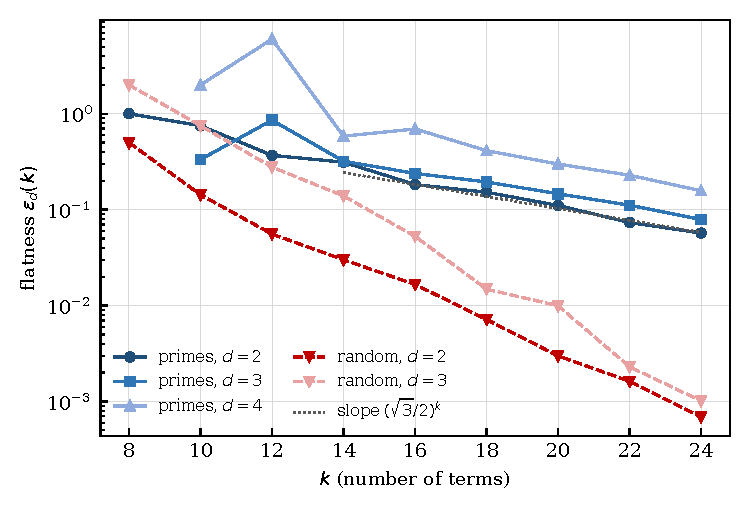
\includegraphics[width=0.82\textwidth]{fig_flatness.pdf}
\caption{Exact flatness $\varepsilon_d(k)$ on a logarithmic scale. The primes
(blue) track the reference slope $(\sqrt3/2)^{k}$ predicted by the modulo-$6$
heuristic of \S\ref{sec:flatness-measured}(i); random odd sequences (red,
median over $20$ seeds) decay strictly faster.}
\label{fig:flatness}
\end{figure}

\begin{table}[htbp]
\centering
\small
\begin{tabular}{rccccc}
\toprule
$d$ & $\lambda(\varepsilon_d)$, primes & $R^2$ &
$\lambda(\text{ripple})$ & $R^2$ & $\lambda(\varepsilon_d)$, random\\
\midrule
2 & 0.8478 & 0.986 & 0.8590 & 0.989 & 0.683\\
3 & 0.8721 & 0.996 & 0.8577 & 0.988 & 0.611\\
4 & 0.8643 & 0.929 & 0.8569 & 0.990 & ---\\
6 & --- & --- & 0.8684 & 0.983 & ---\\
\bottomrule
\end{tabular}
\caption{Decay rate $\lambda$ of $\varepsilon_d(k)$ and of the modulo-$6$
ripple amplitude, from log-linear regression on $k\ge14$. Compare
$\sqrt3/2=0.86603$.}
\label{tab:rates}
\end{table}

Two features stand out.

\emph{(i) The rate matches $\sqrt3/2$.} We have $\sqrt3/2=0.86603$, and the
measured ripple rates lie in $[0.857,0.868]$, i.e.\ within $1.1\%$. Here is the
heuristic that predicts it. Every prime $\ge5$ is $\equiv\pm1\pmod6$.
Consequently the generating polynomial of $B_d$ evaluated at a primitive sixth
root of unity $\zeta$ is $\prod_{a\in B_d}(1+\zeta^{a})$ with each factor of
modulus $|1+\zeta^{\pm1}|=\sqrt3$, against $2$ for the trivial character. The
non-trivial character therefore contributes a ripple of relative amplitude
$(\sqrt3/2)^{|B_d|}$ to $r_{B_d}$, periodic with period $6$. Since
$|B_d|=k-N(d)$ and $N(d)$ is bounded for fixed $d$, the amplitude decays like
$(\sqrt3/2)^{k}$. The measurement confirms both the rate and the period.

\emph{(ii) Random sequences are flatter.} Random odd sequences show
$\lambda\approx0.68$ and $0.61$, i.e.\ strictly faster decay, and at $k=24$
their median $\varepsilon_2$ is $0.0007$ against $0.0570$ for the primes --- a
factor of $80$. The primes are subject to an arithmetic obstruction that generic
sequences are not.

This is the sense in which the primes are simultaneously \emph{smoother} and
\emph{less flat} than random sequences: smoother at first order, because
$\Gamma$ is small (\S\ref{sec:experiments}), but less flat at second order,
because of the modulo-$6$ bias. We isolate the resulting conjecture in
\S\ref{sec:open}.

\section{Numerical experiments}\label{sec:experiments}

\subsection{Setup}

All landscapes below are enumerated exhaustively. For $k\le20$ we used a
compiled Lean executable enumerating all $2^{k}$ configurations (the full
$100$-seed sweep over $k\in\{8,12,16,18,20\}$ takes $11.5$\,s); for $k\le24$ we
used exact dynamic programming over $\mathbb{Z}$ via
Theorem~\ref{thm:stratification}, cross-validated against the enumeration at
$k=20$ (both give $\lm=22808$, $\deg=4344$). Random sequences are drawn without
replacement from the odd integers in $[3,a_k]$, matching the range of the primes
of the same length. The target is $n=\lfloor T/2\rfloor$ throughout.

\subsection{$\lm/\deg$ converges to $\Gamma$}

Put $Q=(\lm/\deg)/\Gamma$. Theorem~\ref{thm:sandwich} predicts
$Q\in[(1+\varepsilon)^{-1},1+\varepsilon]$ up to the negligible tail term.
Table~\ref{tab:Q} and Figure~\ref{fig:convergence} record the behaviour.

\begin{table}[htbp]
\centering
\small
\begin{tabular}{rcccccc}
\toprule
$k$ & mean $Q$ & s.d. & slope $a$ (s.e.) & intercept $b$ & $R^2$ &
$\mathrm{corr}(\Gamma,\lm)$\\
\midrule
8 & 1.112 & 0.498 & 1.907 (0.275) & $-4.757$ & 0.329 & 0.843\\
12 & 1.002 & 0.080 & 1.050 (0.038) & $-0.342$ & 0.884 & 0.956\\
16 & 0.993 & 0.025 & 1.033 (0.014) & $-0.313$ & 0.982 & 0.951\\
18 & 0.992 & 0.014 & 1.028 (0.007) & $-0.281$ & 0.995 & 0.982\\
20 & \textbf{0.995} & \textbf{0.0067} & \textbf{1.013 (0.003)} & $-0.142$ &
\textbf{0.99903} & 0.981\\
\bottomrule
\end{tabular}
\caption{$Q$ over $100$ random odd sequences per $k$; regression of
$\lm/\deg$ on $\Gamma$.}
\label{tab:Q}
\end{table}

\begin{figure}[htbp]
\centering
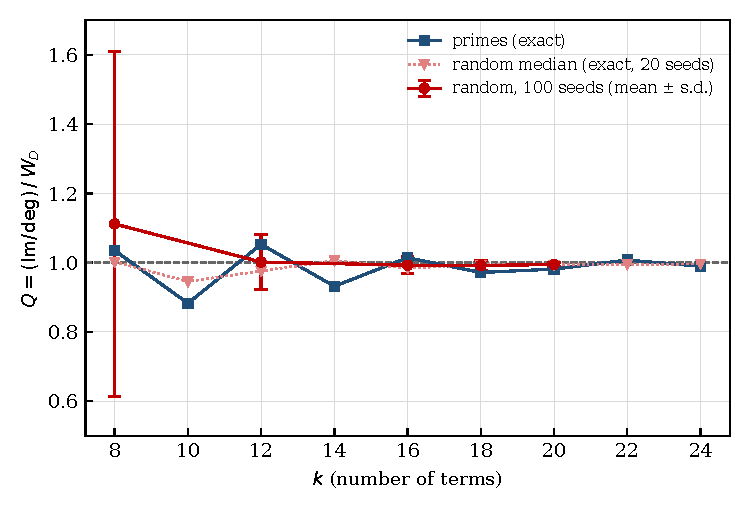
\includegraphics[width=0.82\textwidth]{fig_convergence.pdf}
\caption{Convergence of $Q=(\lm/\deg)/W_D$. Error bars are one standard
deviation over $100$ random sequences; they contract steadily, consistent with
$\varepsilon\to0$. The primes (blue) oscillate about $1$ rather than converging
monotonically; see \S\ref{sec:oscillation} and Conjecture~\ref{conj:oscillation}.}
\label{fig:convergence}
\end{figure}

The dispersion contracts steadily. Correlation between $\Gamma$ and $\lm/\deg$
reaches $0.9995$ at $k=20$.

\subsection{Primes against random}

\begin{table}[htbp]
\centering
\small
\begin{tabular}{lrrrrr}
\toprule
$k$ & 8 & 12 & 16 & 18 & 20\\
\midrule
$z(\lm)$ & $-1.43$ & $-0.96$ & $-1.17$ & $-1.09$ & $-1.14$\\
percentile of $\lm$ & 10 & 21 & 8 & 5 & 4\\
$z(\Gamma)$ & $-0.76$ & $-1.20$ & $-1.30$ & $-1.09$ & $-1.09$\\
\bottomrule
\end{tabular}
\caption{Position of the primes within the $100$ random instances.}
\label{tab:primes-z}
\end{table}

The primes have fewer valleys than a random sequence of the same length and
range at every $k$ tested, but the effect is of size $\approx1$ standard
deviation and is not individually significant. What Table~\ref{tab:primes-z}
does show clearly is that $z(\lm)\approx z(\Gamma)$: whatever smoothness the
primes possess is accounted for by their gap series, exactly as
Theorems~\ref{thm:window} and~\ref{thm:sandwich} predict.

\subsection{An oscillation}\label{sec:oscillation}

The exact computation at $k\le24$ reveals a feature invisible at the resolution
of Table~\ref{tab:Q}. For the primes,
\[
  Q(k)=1.035,\;0.883,\;1.053,\;0.932,\;1.014,\;0.972,\;0.982,\;1.007,\;0.990
  \qquad(k=8,10,\dots,24),
\]
oscillating about $1$ rather than converging monotonically, whereas the median
$Q$ over random instances increases monotonically from below to $0.9967$ at
$k=24$. We believe this oscillation is the signature of the modulo-$6$ ripple of
\S\ref{sec:flatness-measured} beating against the target
$n=\lfloor T/2\rfloor$; see Conjecture~\ref{conj:oscillation}.

\section{Comparison with the coefficient of variation}\label{sec:cv}

Alyahya and Rowe~\cite{AR14} reported that the number of local optima in the
$1$-bit-flip NPP landscape correlates strongly and negatively with the
coefficient of variation $CV=\mathrm{sd}(a)/\mathrm{mean}(a)$ of the weights,
and proposed an estimator on that basis. Using the $100$-seed data of
\S\ref{sec:experiments} we first reproduce their finding, then separate the two
predictors.

\begin{table}[htbp]
\centering
\small
\begin{tabular}{rccccc}
\toprule
$k$ & $\mathrm{corr}(CV,\lm)$ & $\mathrm{corr}(\Gamma,\lm)$ &
$\mathrm{corr}(CV,\Gamma)$ &
$\mathrm{partial}(\Gamma,\lm\mid CV)$ &
$\mathrm{partial}(CV,\lm\mid\Gamma)$\\
\midrule
8 & $-0.874$ & $+0.843$ & $-0.927$ & $+0.178$ & $-0.461$\\
12 & $-0.878$ & $+0.956$ & $-0.907$ & $+0.790$ & $-0.092$\\
16 & $-0.757$ & $+0.951$ & $-0.836$ & $+0.887$ & $+0.225$\\
18 & $-0.741$ & $+0.982$ & $-0.807$ & $+0.967$ & $+0.451$\\
20 & $-0.793$ & $+0.981$ & $-0.838$ & $+0.952$ & $+0.279$\\
\bottomrule
\end{tabular}
\caption{Correlations and partial correlations, $100$ random instances per $k$.}
\label{tab:cv}
\end{table}

For $\lm/\deg$ --- the quantity our theorems actually control --- the separation
is sharper still: at $k=20$,
$\mathrm{partial}(\Gamma,\lm/\deg\mid CV)=+0.9986$
($p=2.4\times10^{-126}$) while
$\mathrm{partial}(CV,\lm/\deg\mid\Gamma)=+0.306$.

For $k\ge12$, conditioning on $CV$ leaves the predictive power of $\Gamma$
essentially intact, whereas conditioning on $\Gamma$ removes most of that of
$CV$. We read this as: $CV$ is a proxy for $\Gamma$, useful because the two are
strongly correlated ($\approx-0.85$) for random sequences, but not the operative
quantity.

This is what Theorem~\ref{thm:window} predicts. $CV$ is a function of the
multiset of weights; $\Gamma$ is not. The window measure $W_D$, being a function
of the multiset, agrees with $\Gamma$ \emph{only for the increasing ordering}
(Example~\ref{ex:order}). Any order-blind statistic must therefore fail to equal
$W_D$ in general, and $CV$ can capture $\Gamma$ only to the extent that, for the
random model in question, order-blind data happen to determine the increasing
rearrangement's gap series in distribution.

A concrete illustration: for the primes, $z(CV)$ is
$+0.85,+1.52,+1.70,+1.51,+1.57$ at $k=8,\dots,20$ --- \emph{positive}, i.e.\ the
primes are more dispersed than random. Both accounts therefore predict ``primes
are smooth'', but only $\Gamma$ predicts the magnitude, and only $\Gamma$
appears in an identity.

\section{Open problems}\label{sec:open}

\begin{problem}[Asymptotic flatness]\label{prob:flatness}
Show that for the sequences of interest the flatness $\varepsilon_k$ of
Definition~\ref{def:flat} tends to $0$, so that
Theorem~\ref{thm:sandwich} yields $\lm_A(n)/\deg_A(n)\to\Gamma(A)$.
\end{problem}

For random odd sequences this appears to be within reach of local central limit
theorems together with Erd\H{o}s--Littlewood--Offord
anticoncentration~\cite{Er45}, which bounds $\max_m r_B(m)$ from above and is
exactly the ingredient needed to control the tail hypothesis. For the primes the
situation is different. The classical asymptotic for partitions into distinct
primes, due to Roth and Szekeres~\cite{RS54}, gives
$\log p(n,\mathcal{P})\sim\kappa\sqrt{2n/\log n}$; \emph{this is a statement on
the logarithmic scale and does not suffice}, since flatness is a statement about
\emph{ratios} of $r$ at nearby arguments. What is required is either an
asymptotic with the pre-exponential factor for distinct-prime partitions of
truncated prime sequences, or a direct exponential-sum estimate of Vinogradov
type for $r_{B_d}$.

\begin{problem}[From residue classes to windows]\label{prob:window-floor}
Transfer Theorem~\ref{thm:floor} from the aggregate counts $R_c$ to the bounded
windows $\mathrm{Win}_d$: show that $\varepsilon_d\gg2^{-|B_d|/2}$ for every odd
sequence, or exhibit a sequence whose window flatness beats the modulus-$4$
scale. The numerics of \S\ref{sec:floor} suggest the former, with the two
quantities agreeing to within a factor $2$ for random sequences; a proof
appears to need the local central limit theorem of
Conjecture~\ref{conj:ripple}, since a bound on residue-class totals says
nothing directly about $O(1)$ many points.
\end{problem}

\begin{conjecture}[Ripple amplitude]\label{conj:ripple}
For the odd primes and fixed $d\ge2$,
\[
  \frac{r_{B_d}(m)}{\mathrm{Main}(m)}-1
  \;=\;2\Bigl(\tfrac{\sqrt3}{2}\Bigr)^{|B_d|+1}
        \cos\Bigl(\tfrac{\pi m}{3}-\tfrac{\pi}{6}(c_1-c_5)\Bigr)
        +o\bigl((\sqrt3/2)^{k}\bigr),
\]
where $\mathrm{Main}$ is the local-CLT Gaussian and
$c_j=\#\{a\in B_d: a\equiv j\bmod 6\}$; consequently
$\varepsilon_d(k)\asymp(\sqrt3/2)^{k}$.
\end{conjecture}

The arithmetic input here is not conjectural. Write $\zeta=e^{2\pi i/6}$ and
$F_B(z)=\prod_{a\in B}(1+z^{a})$, so the $r_B$ are the coefficients of $F_B$.

\begin{proposition}[Character values]\label{prop:character}
$|1+\zeta^{a}|$ depends only on $a\bmod6$, taking the values
$2,\sqrt3,1,0,1,\sqrt3$ for $a\equiv0,\dots,5$. Hence if every element of $B$ is
a prime $\ge5$ then $F_B(\zeta)=3^{|B|/2}e^{i(\pi/6)(c_1-c_5)}$, so that
$|F_B(\zeta)|/2^{|B|}=(\sqrt3/2)^{|B|}$ \emph{exactly}; if $3\in B$ then
$F_B(\zeta)=0$; and $F_B(-1)=0$ for any odd $B$, which is
Theorem~\ref{thm:no-flat} in Fourier form.
\end{proposition}

\begin{proof}
$|1+e^{i\pi a/3}|^{2}=2+2\cos(\pi a/3)$ takes the stated values. Every prime
$\ge5$ is $\equiv\pm1\pmod6$ and $1+\zeta^{\pm1}=\sqrt3\,e^{\pm i\pi/6}$;
multiplying gives the formula. For $a\equiv3$ the factor $1+\zeta^{3}$ vanishes,
and $\zeta^{3}=-1$ gives the last claim.
\end{proof}

What remains conjectural is only the transfer from this Fourier datum to
pointwise ratios. The exponent $|B_d|+1$ rather than $|B_d|$ comes from the
width factor $\sqrt{V_0/V_6}=\sqrt3/2$ at the sub-arc, where
$V_0=\tfrac14\sum a^{2}$ and $V_6=\tfrac14\sum a^{2}\sec^{2}(\pi a/6)
=\tfrac13\sum a^{2}$. We have tested both parts numerically for $k\le32$ by
extracting the period-$6$ Fourier component of $r_{B_d}/\mathrm{Main}-1$.

The measured phase agrees with $(\pi/6)(c_1-c_5)$ to four decimal places,
including at $k=16$, where $c_1-c_5=-3$ moves the predicted phase to $-\pi/2$.

For the amplitude, the extraction is sensitive to the width of the window over
which the Fourier component is taken, because the Gaussian reference degrades in
the tails: at $k=26$ the ratio to $2(\sqrt3/2)^{|B_d|+1}$ is
$0.972,\,0.991,\,1.056$ for half-widths $24,\,90,\,180$ respectively, while
$\sigma=\sqrt{V_0}\approx147$. Taking a narrow window (half-width $24$, about
$0.15\sigma$, still eight full periods) the ratio is stable in the window and
approaches $1$; the corresponding ratios to $2(\sqrt3/2)^{|B_d|}$ move
\emph{away} from $1$, which is what identifies the extra factor $\sqrt3/2$.

The approach to $1$ splits into two branches according to the value of
$c_1-c_5$, which is also the phase:
\[
\begin{array}{llll}
  c_1-c_5=-1: & 0.965,\,0.968,\,0.970,\,0.972,\,0.974,\,0.976,\,0.981,\,0.981
    & (k=20,\dots,30,36,38) & \text{from below},\\[2pt]
  c_1-c_5=-3: & 1.025,\,1.019,\,1.015
    & (k=32,34,40) & \text{from above}.
\end{array}
\]
Both branches converge to $1$, from opposite sides. Since the phase itself is
reproduced to within $7\times10^{-4}$ in both branches, the residual is not an
error in the phase but a \emph{phase-coupled} correction to the amplitude ---
which is what one expects from interference between the leading sub-arc term and
the next one. We regard this as evidence for
Conjecture~\ref{conj:ripple} and as a constraint on any refinement of it.

We have also verified the width factor at a second modulus. For $q=4$ the
prediction is $\sqrt{V_0/V_4}=1/\sqrt2$, and measuring the period-$4$ component
on the stratum $d=1$ of the primes (where $3\in B_1$ kills the period-$6$ mode)
gives ratios $0.91$--$0.97$ to the prediction \emph{with} the width factor
against $0.64$--$0.69$ \emph{without} it; for random odd sequences the
corresponding medians are $\approx1.05$ and $\approx0.75$. The modulus $q=3$
cannot be tested this way: for any odd sequence coprime to $3$ one has
$\rho_3=(1/2)^{|B|}$, which is dominated by $\rho_4=(1/\sqrt2)^{|B|}$, so the
period-$3$ component never rises above the period-$4$ one.

\begin{proposition}[Extremality of the modulus $6$]\label{prop:mod6}
Let $M(q)$ denote the geometric mean of $|\cos(\pi r/q)|$ over the $r$ coprime
to $q$. Then
\[
  M(q)=\tfrac12\,|\Phi_q(-1)|^{1/\varphi(q)},
\]
where $\Phi_q$ is the $q$-th cyclotomic polynomial, and
\[
  \sup_{q\ge3}M(q)=\frac{\sqrt3}{2},
\]
attained at $q=6$ and nowhere else. The next largest values are
$M(10)=5^{1/4}/2$, $M(4)=1/\sqrt2$ and $M(14)=7^{1/6}/2$.
\textup{(Lean, finite part: \Lean{M12\_six\_maximal}, \Lean{M12\_gap}.)}
\end{proposition}

\begin{proof}
Since $\prod_{r\perp q}(x-\zeta_q^{r})=\Phi_q(x)$, evaluating at $x=-1$ and
using $|1+\zeta_q^{r}|=2|\cos(\pi r/q)|$ gives
$|\Phi_q(-1)|=2^{\varphi(q)}\prod_{r\perp q}|\cos(\pi r/q)|$, which is the
identity. For the supremum use the classical values: $\Phi_q(-1)=p$ when
$q=2p^{j}$ with $p$ an odd prime, $\Phi_q(-1)=2$ when $q=2^{j}$ with $j\ge2$,
and $\Phi_q(-1)=1$ for all other $q\ge3$. Hence $M(q)=1/2$ except in two
families. For $q=2p^{j}$ we get $M(q)=\tfrac12p^{1/(p^{j-1}(p-1))}$, which is
largest when the exponent is largest, i.e.\ at $j=1$; and
$p\mapsto p^{1/(p-1)}$ decreases on odd primes ($3^{1/2}>5^{1/4}>7^{1/6}>\cdots$),
so the family is maximised at $q=6$ with value $\sqrt3/2$, the runner-up being
$q=10$. For $q=2^{j}$, $j\ge2$, we get $M(q)=\tfrac12\cdot2^{1/2^{j-1}}$,
maximised at $j=2$ with value $1/\sqrt2<\sqrt3/2$.
\end{proof}

We verified the identity numerically for $3\le q\le40$ to machine precision,
obtaining $M(6)=0.866025$, $M(10)=0.747674$, $M(4)=0.707107$,
$M(14)=0.691544$. The finite comparison is also formalised: raising to the
twelfth power clears denominators, giving $729,125,64,49,8$ over $4096$ for
$q=6,10,4,14,8$ and $1/4096$ otherwise, so the maximality of $q=6$ reduces to a
comparison of rationals.

The number-theoretic content is this. For a sequence equidistributed among the
residues coprime to $q$, $M(q)$ is the decay rate of $|F_B(\zeta_q)|/2^{|B|}$;
Proposition~\ref{prop:mod6} then says that $q=6$ is the slowest mode available
to any such sequence. The primes are confined to exactly two residues modulo
$6$, both of which realise the maximal $|\cos|$, and no other modulus offers a
comparable concentration --- which is why the bias modulo $6$, and no other
congruence obstruction, governs the flatness of the primes. The step from
equidistribution to the decay rate is the one genuinely analytic ingredient
here, and we do not prove it; see Problem~\ref{prob:flatness}.

\begin{conjecture}[Oscillation]\label{conj:oscillation}
The oscillation of $Q(k)$ for the primes observed in \S\ref{sec:oscillation} is
caused by the ripple of Conjecture~\ref{conj:ripple} beating against
$n=\lfloor T/2\rfloor$. Precisely, writing $A_d,\varphi_d$ for the amplitude and
phase in Conjecture~\ref{conj:ripple} and
$P_d=\prod_{a\in I_d}(1+e^{-i\pi a/3})$,
\[
  \frac{\lm_A(n)}{\deg_A(n)}-W_D(A)\;\approx\;
  \sum_{d\ge1}2^{-N(d)}\,\mathrm{Re}\Bigl[A_de^{-i\varphi_d}
  \bigl(e^{i\pi(n+d)/3}+e^{i\pi(n-d-\sigma_d)/3}
        -2e^{i\pi n/3}P_d2^{-N(d)}\bigr)\Bigr].
\]
\end{conjecture}

Evaluating the right-hand side for $k\le26$ reproduces the sign of the observed
deviation in $9$ of the $10$ cases (all but $k=8$) and its magnitude to within a
factor $0.5$--$1.7$, with a systematic under-estimate of about $25\%$ that we
attribute to higher-order sub-arc corrections. The stratum $d=2$ dominates, and
$d=1$ contributes exactly zero because $3\in B_1$ forces $F_{B_1}(\zeta)=0$ by
Proposition~\ref{prop:character} --- which also explains why $\varepsilon_1$ is
two orders of magnitude below $\varepsilon_2$ in Table~\ref{tab:flatness}.

We warn against the simpler guess that the sign is governed by $T\bmod6$ alone:
for the primes $T\equiv2\pmod6$ throughout $k=8,\dots,14$ and $k=18,\dots,26$,
yet the sign of the deviation alternates across that range. The dependence on
$c_1-c_5$ and on $\sigma_d$ in the displayed formula is essential.

\begin{problem}[Asymptotic smoothness of the primes]\label{prob:primes}
Determine whether $\lm_{P_k}(n)/\lm_{R_k}(n)\to0$ as $k\to\infty$, where $P_k$
is the first $k$ odd primes and $R_k$ a random odd sequence of the same length
and range. By Theorem~\ref{thm:sandwich} this reduces to comparing
$\Gamma(P_k)$, which converges (to $\approx5.3493$), with
$\mathbb{E}[\Gamma(R_k)]$, which we expect to grow like twice the mean gap,
i.e.\ $\asymp\log k$.
\end{problem}

\begin{problem}[Off-centre targets]\label{prob:rho}
For $n/T=\rho\ne1/2$ the factor $2^{-N(d)}$ in the window series is replaced by
$(1-\rho)^{N(d)}$, deforming $\Gamma$ into the family
$\Gamma_x(A)=\sum_j a_jx^{j}$ evaluated at $x=1-\rho$. Develop the corresponding
theory, including the large-deviation rate function that governs $\lm/2^{k}$
away from the centre.
\end{problem}

\begin{thebibliography}{XXXX}

\bibitem[AR14]{AR14}
K.~Alyahya and J.~E.~Rowe,
\emph{Local optima and weight distribution in the number partitioning problem},
in: Parallel Problem Solving from Nature --- PPSN XIII,
Lecture Notes in Computer Science \textbf{8672}, Springer, Cham, 2014,
pp.~862--871. \href{https://doi.org/10.1007/978-3-319-10762-2_85}{DOI:10.1007/978-3-319-10762-2\_85}.

\bibitem[Ba21]{Ba21}
P.~Barry,
\emph{On the gap-sum and gap-product sequences of integer sequences},
preprint (2021), \href{https://arxiv.org/abs/2104.05593}{arXiv:2104.05593}.

\bibitem[BCP01]{BCP01}
C.~Borgs, J.~T.~Chayes and B.~Pittel,
\emph{Phase transition and finite-size scaling for the integer partitioning
problem}, Random Structures \& Algorithms \textbf{19} (2001), no.~3--4,
247--288. \href{https://doi.org/10.1002/rsa.10004}{DOI:10.1002/rsa.10004}.

\bibitem[Er45]{Er45}
P.~Erd\H{o}s, \emph{On a lemma of Littlewood and Offord},
Bulletin of the American Mathematical Society \textbf{51} (1945), 898--902.

\bibitem[FF98]{FF98}
F.~F.~Ferreira and J.~F.~Fontanari,
\emph{Probabilistic analysis of the number partitioning problem},
Journal of Physics A: Mathematical and General \textbf{31} (1998), no.~15,
3417--3428.
\href{https://doi.org/10.1088/0305-4470/31/15/007}{DOI:10.1088/0305-4470/31/15/007}.

\bibitem[Me01]{Me01}
S.~Mertens, \emph{A physicist's approach to number partitioning},
Theoretical Computer Science \textbf{265} (2001), no.~1--2, 79--108.
\href{https://doi.org/10.1016/S0304-3975(01)00153-0}{DOI:10.1016/S0304-3975(01)00153-0}.

\bibitem[RS54]{RS54}
K.~F.~Roth and G.~Szekeres,
\emph{Some asymptotic formulae in the theory of partitions},
The Quarterly Journal of Mathematics \textbf{5} (1954), no.~1, 241--259.
\href{https://doi.org/10.1093/qmath/5.1.241}{DOI:10.1093/qmath/5.1.241}.

\bibitem[SHF03]{SHF03}
P.~F.~Stadler, W.~Hordijk and J.~F.~Fontanari,
\emph{Phase transition and landscape statistics of the number partitioning
problem}, Physical Review E \textbf{67} (2003), 056701.

\end{thebibliography}

\appendix

\section{The Lean development}\label{app:lean}

The formalisation targets Lean~4 (toolchain \Lean{leanprover/lean4:v4.32.2})
with Mathlib pinned to the matching tag. Building with \Lean{lake build}
verifies every declaration below. Each is checked with \Lean{\#print axioms} to
depend only on \Lean{propext}, \Lean{Classical.choice} and \Lean{Quot.sound};
no declaration depends on \Lean{sorryAx}.

\begin{center}
\small
\begin{tabular}{lll}
\toprule
Paper & Lean declaration & File\\
\midrule
Prop.~\ref{prop:bridge} & \Lean{mem\_subsetSums\_ofFn\_iff} & \Lean{Theory/Bridge.lean}\\
Prop.~\ref{prop:gs-min} & \Lean{gs\_ofFn\_eq\_energy\_min} & \Lean{Theory/Bridge.lean}\\
Prop.~\ref{prop:representability} & \Lean{gs\_eq\_zero\_iff} & \Lean{Theory/Symmetry.lean}\\
Thm.~\ref{thm:classification} & \Lean{isStrictLocalMin\_iff\_of\_ge} etc. & \Lean{Theory/Landscape.lean}\\
Cor.~\ref{cor:ground-is-min} & \Lean{isStrictLocalMin\_of\_exact} & \Lean{Theory/Landscape.lean}\\
Cor.~\ref{cor:lm-arithmetic} & \Lean{lm\_eq\_lmClassCount} & \Lean{Theory/Landscape.lean}\\
Thm.~\ref{thm:reflection} & \Lean{gs\_compl}; \Lean{lm\_compl} & \Lean{Theory/Landscape.lean}; \Lean{Theory/Symmetry.lean}\\
Thm.~\ref{thm:no-flat} & \Lean{no\_flat\_edge} & \Lean{Theory/Symmetry.lean}\\
Cor.~\ref{cor:strict-eq-weak} & \Lean{isStrictLocalMin\_iff\_le\_of\_odd} & \Lean{Theory/Symmetry.lean}\\
Thm.~\ref{thm:window} & \Lean{windowSeries\_eq\_gapSeries} & \Lean{Theory/Bridge.lean}\\
Lem.~\ref{lem:fibers} & \Lean{fiber\_over}, \Lean{fiber\_under} & \Lean{Theory/Decomposition.lean}\\
Lem.~\ref{lem:vanishing} & \Lean{overCount\_eq\_zero} etc. & \Lean{Theory/Decomposition.lean}\\
Thm.~\ref{thm:stratification} & \Lean{lm\_eq\_sum\_strata}, \Lean{lm\_eq\_lmPartial} & \Lean{Theory/Decomposition.lean}, \Lean{Theory/Total.lean}\\
Thm.~\ref{thm:fiber-rep} & \Lean{fiber\_card\_eq\_repCount} & \Lean{Theory/Fiber.lean}\\
Cor.~\ref{cor:deg-rep} & \Lean{degCount\_eq\_sum\_repCount} & \Lean{Theory/Fiber.lean}\\
Cor.~\ref{cor:strata-rep} & \Lean{overCount\_eq\_repCount} etc. & \Lean{Theory/Sandwich.lean}\\
Lem.~\ref{lem:flat-ratio} & \Lean{ratio\_bounds\_of\_flat} & \Lean{Theory/Sandwich.lean}\\
Thm.~\ref{thm:sandwich} & \Lean{sandwich\_partial}, \Lean{sandwich\_total} & \Lean{Theory/Sandwich.lean}, \Lean{Theory/Total.lean}\\
Thm.~\ref{thm:floor}(i) & \Lean{normSq\_one\_add\_I\_pow\_odd} & \Lean{Theory/Ripple.lean}\\
Thm.~\ref{thm:floor}(iii) & \Lean{max\_abs\_cos\_sin\_sq\_ge}, \Lean{spread\_lower\_bound} & \Lean{Theory/Ripple.lean}\\
Prop.~\ref{prop:mod6} (finite) & \Lean{M12\_six\_maximal}, \Lean{M12\_gap} & \Lean{Theory/Ripple.lean}\\
Prop.~\ref{prop:character} & \Lean{normSq\_one\_add\_exp} and specialisations & \Lean{Theory/Ripple.lean}\\
\bottomrule
\end{tabular}
\end{center}

The development also contains machine-checked numerical cross-checks
(\Lean{\#eval}), among them: the identity of Theorem~\ref{thm:stratification}
for $A=(3,5,7,11,13,17)$ at every $n\le56$; the coincidence of the strict and
weak local-minimum counts for the same $A$
(Corollary~\ref{cor:strict-eq-weak}); the window identity for the first twenty
odd primes, both sides evaluating to $1402281/262144$; and the failure of that
identity for the reordering $(5,3)$ of Example~\ref{ex:order}.

\end{document}
